\documentclass{article}
\usepackage[utf8]{inputenc}
\usepackage{polski}
\usepackage{graphicx}
\usepackage{fancyhdr}
\usepackage{lastpage}
\usepackage{listings}
\usepackage[T1]{fontenc}


\pagestyle{fancy}

\fancyhf{}

\fancyfoot[C]{\thepage\ / \pageref{LastPage}} % Ustawienie numeracji stron w stopce

\fancypagestyle{plain}{ % Nadpisanie stylu strony tytułowej
    \fancyhf{}
    \renewcommand{\headrulewidth}{0pt} % Usunięcie nagłówka
    \fancyfoot[C]{\thepage\ / \pageref{LastPage}}
}

\title{Sprawozdanie końcowe projekt 1 w C}
\author{Sebastian Grosfeld i Miłosz Mertka }
\date{\today}

 \lstdefinestyle{tree}{
    literate=
    {├}{{\smash{\raisebox{-1ex}{\rule{1pt}{\baselineskip}}}\raisebox{0.5ex}{\rule{1ex}{1pt}}}}1 
    {─}{{\raisebox{0.5ex}{\rule{1.5ex}{1pt}}}}1 
    {└}{{\smash{\raisebox{0.5ex}{\rule{1pt}{\dimexpr\baselineskip-1.5ex}}}\raisebox{0.5ex}{\rule{1ex}{1pt}}}}1 
  }

\begin{document}

\maketitle

\tableofcontents

\newpage

% Poniżej ustawiany jest nagłówek
\setlength{\headheight}{23pt}
\lhead{Miłosz Mertka\\Sebastian Grosfeld}
\rhead{Sprawozdanie końcowe\\projektu 1 w języku C}

\maketitle

\section{Wprowadzenie}
    Celem projektu jest stworzenie programu, który będzie w stanie wykonać następujące zadania:
\begin{enumerate}
    \item Wygeneruje graf w postaci siatki (\emph{Rysunek \ref{fig:wagi}}) o podanej liczbie kolumn i wierszy. Krawędzie i wagi krawędzi losowane są w podanym zakresie wartości.
    \item Zapisze taki graf do pliku o ustalonym formacie.
    \item Przeczyta z pliku o ustalonym formacie taki graf.
    \item Potrafi określić za pomocą algorytmu BFS, czy dany graf jest spójny.
    \item Potrafi wyznaczyć w tym grafie najkrótsze ścieżki pomiędzy wybranymi parami wierzchołków, korzystając z algorytmu Dijkstry.
\end{enumerate}
\begin{figure}[htp]
        \centering
        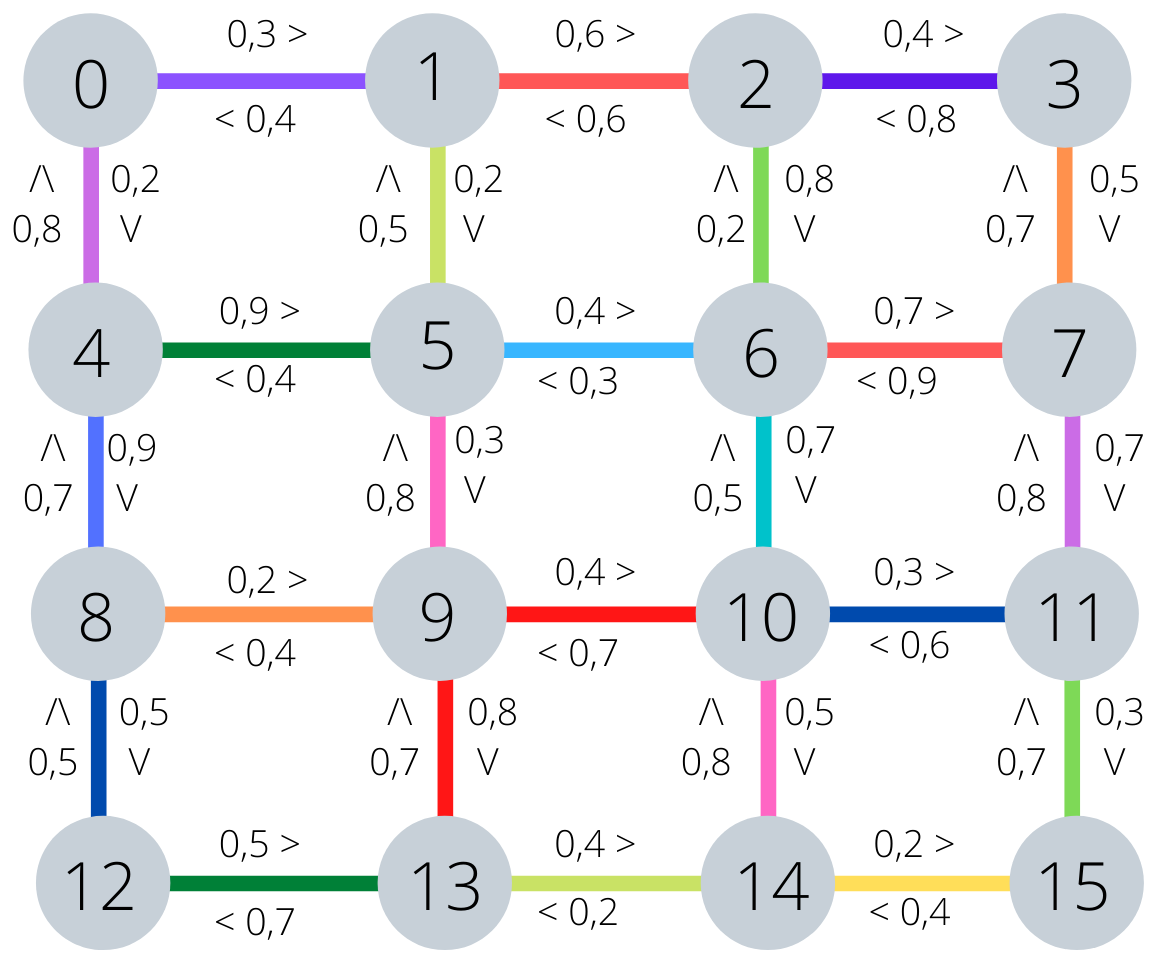
\includegraphics[width=7cm]{images/wagi.png}
        \caption{Wizualizacja przykładowego, wygenerowanego grafu}
        \label{fig:wagi}
\end{figure}
\textbf{Graf} definiuje się następująco: $G=(V,E)$. $V$ jest zbiorem wierzchołków grafu, $E$ jest zbiorem jego krawędzi.
\vspace{5mm}
\\
\textbf{Algorytm BFS} nazywany jest algorytmem \emph{przeszukiwania grafu wszerz}.\linebreak W projekcie znajduje on zastosowanie przy sprawdzaniu, czy dany graf jest spójny.
\vspace{5mm}
\\
\textbf{Algorytm Dijkstry} służy do wyznaczania najkrótszych ścieżek od wierzchołka źródłowego do wszystkich innych wierzchołków grafu. Algorytm działa wyłącznie dla grafów ważonych, którego wagi są nieujemne. W projekcie narzucony został także dodatkowy wymóg spójności danego grafu, aby mieć pewność,\linebreak że algorytm Dijkstry znajdzie zadane ścieżki.
\section{Aktualny stan projektu}
\subsection{Struktura katalogów}

W głównym katalogu projektu znajdują się także dwa podkatalogi. Podkatalog \emph{documentation} zawiera dokumentację związaną z projektem, z kolei \emph{test\textunderscore files} zawiera pliki wykorzystywane w testach (ich opis został zawarty w \emph{Specyfikacji funkcjonalnej projektu 1 w języku C}, która znajduje się w pliku \emph{Specyfikacja\textunderscore funkcjonalna.pdf}). W pliku \textbf{Makefile} zaimplementowane zostały testy jednostkowe oraz pomocnicze instrukcje do kompilowania kodu.


\begin{lstlisting}[style=tree]
.
├── bfs.c
├── bfs.h
├── constants.h
├── dijkstra.c
├── dijkstra.h
├── documentation
│   ├── functional_specification.tex
│   ├── images
│   │   ├── directed_graph.png
│   │   ├── graf_pp.png
│   │   ├── graph_inconsistent.png
│   │   ├── graph.png
│   │   ├── graph_weights.png
│   │   ├── modulo.png
│   │   └── wagi.png
│   └── implementation_specification.tex
├── generate.c
├── generate.h
├── graph.c
├── graph.h
├── handle_files.c
├── handle_files.h
├── help.c
├── help.h
├── main.c
├── Makefile
├── random.c
├── random.h
├── test_bfs.c
├── test_dijkstra.c
├── test_files
│   ├── cos_graph.txt
│   ├── dijkstra_test_expected.txt
│   ├── incos_graph.txt
│   ├── t_graph.txt
│   └── wf_graph.txt
├── test_graph.c
├── test_handle_files.c
├── test_validate_input.c
├── validate_input.c
└── validate_input.h
\end{lstlisting}

\newpage

\subsection{Instrukcje uruchomienia}

Aby poprawnie obsługiwać program należy znać jego tryby pracy oraz argumenty, jakie dla poszczególnych trybów należy podać. W przypadku podania nieprawidłowych argumentów zostanie wyświetlony odpowiedni komunikat o błędzie. Poniżej znajdują się składnie dla poszczególnych trybów oraz przykłady ich uruchomienia. Aby wywołać pomoc do programu, należy w miejsce podawania trybu podać wartość \emph{help}.

\medskip

\subsubsection{Tryb generate\textunderscore wages}
Składnia:\\
\textit{nazwa\textunderscore programu tryb\textunderscore działania nazwa\textunderscore pliku liczba\textunderscore wierszy liczba\textunderscore kolumn waga\textunderscore od waga\textunderscore do}

\medskip

\noindent Przykład:\\
\textit{./grapher generate\textunderscore wages graf.txt 8 5 1 3}\\
Wywołanie powyższego polecenia spowoduje wygenerowanie grafu ze wszystkimi krawędziami o losowych wagach. Wagi są losowane z przedziału $<1, 3>$. Wygenerowane zostanie 8 wierszy i 5 kolumn. Wynikowy graf zostanie zapisany do pliku \emph{graf.txt}.

\subsubsection{Tryb generate\textunderscore consistent}
Składnia:\\
\textit{nazwa\textunderscore programu tryb\textunderscore działania nazwa\textunderscore pliku liczba\textunderscore wierszy liczba\textunderscore kolumn waga\textunderscore od waga\textunderscore do}

\medskip

\noindent Przykład:\\
\textit{./grapher generate\textunderscore consistent graf.txt 7 6 1 2}\\
Wywołanie powyższego polecenia spowoduje wygenerowanie grafu spójnego\linebreak o lososwych wagach krawędzi z przedziału $<1, 2>$. Wygenerowane zostanie 7 wierszy i 6 kolumn. Wynikowy graf zostanie zapisany do pliku \emph{graf.txt} .

\subsubsection{Tryb generate\textunderscore random}
Składnia:\\
\textit{nazwa\textunderscore programu tryb\textunderscore działania nazwa\textunderscore pliku liczba\textunderscore wierszy liczba\textunderscore kolumn waga\textunderscore od waga\textunderscore do}

\medskip

\noindent Przykład:\\
\textit{./grapher generate\textunderscore random graf.txt 12 15 2 8}\\
Wywołanie powyższego polecenia spowoduje wygenerowanie grafu o losowych wagach i krawędziach (\emph{brak gwarancji spójności grafu}). Wagi są losowane z przedziału $<2, 8>$. Wygenerowane zostanie 12 wierszy i 15 kolumn. Wynikowy graf zostanie zapisany do pliku \emph{graf.txt}.

\newpage

\subsubsection{Tryb analyze}
Składnia:\\
\textit{nazwa\textunderscore programu tryb\textunderscore działania nazwa\textunderscore pliku  [droga\textunderscore źródło] [droga\textunderscore cel] [droga\textunderscore źródło(1)] [droga\textunderscore cel(1)]}

\medskip

\noindent Przykład:\\
\textit{./grapher analyze graf.txt 16 8}\\
Wywołanie powyższego polecenia spowoduje analizę grafu z pliku \emph{graf.txt} pod kątem jego spójności. Dodatkowo program spróbuje znaleźć najkrótszą ścieżkę od wierzchołka 16 do wierzchołka 8.

\subsection{Wymagania funkcjonalne}
Program potrafi:
\begin{itemize}
    \item Wczytać ze wskazanego pliku i przeanalizować graf zapisany w pliku\linebreak o ustalonym formacie pod kątem spójności oraz (jeśli spełnia on określone warunki) wyznaczyć najkrótsze ścieżki między określonymi wierzchołkami.
    \item Wygenerować graf według wybranego trybu generacji oraz zapisać go\linebreak w ustalonym formacie do wskazanego pliku.
\end{itemize}
\subsection{Wymagania niefunkcjonalne}
Program:
\begin{itemize}
    \item jest wsadowy (nie oczekuje interakcji z użytkownikiem po uruchomieniu),
    \item uruchamia się na maszynach studenckich w IETiSIP PW z systemem operacyjnym \textbf{Ubuntu 18.04 LTS},
    \item jest napisany w języku C, 
    \item jest uruchamiany z poziomu konsoli.
\end{itemize}

\newpage
\subsection{Testowanie}
Testowanie poszczególnych fukcjonalności odbywa się automatycznie dzięki użyciu narzędzia \textbf{Makefile}. Aby uruchomić ogólny test należy wpisać w konsoli \emph{make test}.
Uruchomią się wtedy poszczególne testy po kolei. Najpierw wyświetlana jest informacja, co powinno się stać. Następnie program przeprowadza test i wyświetla komunikat towarzyszący testowi, jeśli taki istnieje. Na koniec wyświetlana jest informacja czy test wykonał się pomyślnie.\\
Poniżej znajduje się fragment komunikatu testu ogólnego, a zarazem test sprawdzający odpowiedni format pliku.
\vspace{5mm}
\\
\textit{It should print error on wrong file format}\\
\textit{Invalid file format}\\
\textit{Test passed}\\
\vspace{5mm}
\\
Pozostałe testy uruchamiamy nastęującymi komendami:
\begin{itemize}
    \item \emph{test\textunderscore file} -- test operacji na plikach,
    \item \emph{test\textunderscore bfs} -- test algorytmu przeszukiwania grafu wszerz -- BFS,
    \item \emph{test\textunderscore dijkstra} -- test algorytmu Dijkstry,
    \item \emph{test\textunderscore graph} -- test generowania grafu,
    \item \emph{test\textunderscore arguments} -- test reakcji programu na nieprawidłowe argumenty wywołania.
\end{itemize}

\newpage
\section{Przykładowe wyniki}

Poniżej zostały przedstawione przykładowe wyniki dla różnych trybów działania programu.

\medskip
\begin{itemize}
\item \textbf{./grapher help} -- wyświetla pomoc podręczną do obsługi programu.
\vspace{5mm}
\\
\begin{lstlisting}
Grapher is a software that can generate 
graph and analyze them

Usage

There are 4 work modes: generate_wages, 
generate_consistent, generate_random, analyze

Usage for generate_wages mode:
./grapher generate_wages filename rows columns
min_wage max_wage

Usage for generate_consistent mode:
./grapher generate_consistent filename rows columns 
min_wage max_wage

Usage for generate_random mode:
./grapher generate_random filename rows columns 
min_wage max_wage

Usage for analyze mode:
./grapher analyze filename [source] [destination] 
[source(1)] [destination(2)] ...

\end{lstlisting}

\newpage
\item \textbf{./grapher generate\textunderscore wages graf1.txt 4 4 1 5} -- generuje graf z wszystkimi krawędzami i losowymi wagami krawędzi z danego przedziału i zapisuje go do pliku.
   \vspace{3mm}
\\
Zawartość pliku \emph{graf1.txt}:
\begin{lstlisting}
4 4
        1 :2.109447  4 :4.352982
        0 :2.588354  2 :3.427905  5 :3.947031
        1 :1.103453  3 :3.901337  6 :4.360410
        2 :3.834280  7 :2.535106
        0 :3.222548  5 :1.210554  8 :4.182457
        1 :4.862316  4 :3.041101  6 :3.223622  9 :3.001072
        2 :1.841887  5 :3.331970  7 :2.093099  10 :3.919180
        3 :2.664537  6 :1.634950  11 :1.874733
        4 :3.652635  9 :4.492666  12 :2.023580
        5 :2.688648  8 :2.542669  10 :4.358189  13 :3.102860
        6 :4.691214  9 :1.467636  11 :2.041630  14 :3.895540
        7 :4.794667  10 :4.988660  15 :2.796877
        8 :3.628947  13 :4.349070
        9 :1.851495  12 :4.331983  14 :4.559624
        10 :4.075117  13 :3.514441  15 :2.600725
        11 :4.601797  14 :3.376757
\end{lstlisting}
\item \textbf{./grapher generate\textunderscore consistent graf2.txt 3 3 1 2} -- generuje graf spójny z losowymi wagami krawędzi z danego przedziału i zapisuje go do pliku. 
   \vspace{3mm}
\\
Komunikat:
\begin{lstlisting}
consistent
\end{lstlisting}

Zawartość pliku \emph{graf2.txt}:

\begin{lstlisting}
3 3
        1 :1.789364  3 :1.618629
        0 :1.581889  2 :1.862758  4 :1.358315
        1 :1.950590  5 :1.262803
        0 :1.919111  4 :1.679392  6 :1.591066
        1 :1.696167  5 :1.394398  7 :1.052817
        2 :1.594559  4 :1.125758  8 :1.258477
        3 :1.740731  7 :1.327168
        6 :1.324737  8 :1.478851
        5 :1.484448  7 :1.604386
\end{lstlisting}
\newpage
\item \textbf{./grapher generate\textunderscore random graf3.txt 3 3 1 9} -- generuje graf bez gwarancji jego spójności z losowymi wagami krawędzi z danego przedziału i zapisuje go do pliku.
   \vspace{3mm}
\\
Zawartość pliku \emph{graf3.txt}:
\begin{lstlisting}
3 3
        1 :1.466600  3 :5.727846
        0 :5.797210  2 :3.053808  4 :3.482689
        5 :3.944589
        0 :7.965151  6 :7.396492
        1 :5.524738  3 :4.559672  5 :6.657537  7 :7.062099
        2 :7.436613  4 :7.704329  8 :8.505508
        3 :5.233354
        4 :1.771792  6 :8.954748  8 :3.059252
        5 :1.289811  7 :1.197478
\end{lstlisting}
\item \textbf{./grapher analyze graf3.txt 1 4} -- analizuje graf z pliku pod względem spójności oraz jeśli ta została potwierdzona, to wyznacza najkrótszą ścieżkę między wskazanymi wierzchołkami.
   \vspace{3mm}
\\
Komunikat: 
\begin{lstlisting}
consistent

(1, 4) : 1->4
Cost: 3.48269
\end{lstlisting}
\item \textbf{./grapher analyze test\textunderscore files/incos\textunderscore graph.txt 1 4}
   \vspace{3mm}
\\
Komunikat: 
\begin{lstlisting}
inconsistent

\end{lstlisting}
\end{itemize}

\newpage
\section{Lista zmian}

Pełna lista zmian, których dokonaliśmy względem specyfikacji implementacyjnej oraz specyfikacji funkcjonalnej.

\begin{itemize}
    \item Tryb generujący \textbf{generate\textunderscore consistent} przyjmuje argumenty odpowiedzialne za przedział losowania wag krawędzi.
    \item Wyznaczanie najkrótszej ścieżki między wierzchołkami zostało ograniczone do trybu \textbf{analyze} i tylko dla grafów spójnych. 
    \item Został dodany moduł \textbf{help} zawierający pomoc do obsługi programu.\linebreak Używa się go podając w miejsce trybu wartość \emph{help}.
    \item Komunikaty o błedach są teraz bardziej szczegółowe (np. wyświetla jakiego typu powinny być argumenty i wyświetla podręczną pomoc ( tzw. \emph{helpa}))
    \item Zostały dodane nowe stałe. Wszystkie stałe są teraz zawarte w pliku\linebreak \emph{constants.h} .
    \item Testy są teraz przeprowadzane w bardziej oczywisty sposób. Jest teraz wyświetlana informacja o tym, czy test przebiegł pomyślnie czy nie. 
    \item Funkcja \textbf{read\textunderscore file} nie zwracała wcześniej żadnej wartości, a teraz zwraca typ \textbf{graph\textunderscore t*}.
    \item Funkcje \textbf{write\textunderscore file} oraz \textbf{find\textunderscore path} nie zwracały wcześniej żadnej wartości, a teraz zwracają \textbf{int} -- ułatwia to obsługę błędów w programie.
    \item Została dodana nowa funkcja \textbf{initialize\textunderscore rand} przyjmująca jako argumenty minimalną i maksymalną wagę, która zwraca wartość typu\linebreak \textbf{random\textunderscore data\textunderscore t*}.
    \item W strukturze przechowującej graf została zdefiniowana nowa zmienna typu \textbf{int} o nazwie \textbf{nodes\textunderscore count} przechowująca iloczyn liczby wierszy\linebreak oraz kolumn.
    \item Zostały poprawione pliki przechowujące grafy, które są używane w testach.
    \item Uległa zmianie wyświetlana ścieżka w trybie \textbf{analyze}. Teraz nie pokazuje wag przy każym przejściu tylko wyświetla sumę wag z odwiedzonych ścieżek.
\end{itemize}

\section{Współpraca podczas projektu}
Współpraca podczas prac nad projektem składała się na regularne spotkania członków zespołu, podczas których wymieniali się poglądami, wizją oraz pomysłami związanymi z zagadnieniami projektowymi, a także wspólnie pracowali nad dokumentacją i kodem. Jej drugą częścią było wspólne pracowanie na repozytorium oraz wzajemna kontrola kodu. Dowodem na to są chociażby commity widoczne w logach w zdalnym repozytorium.
\section{Wnioski końcowe}
Podczas wspólnej pracy nad projektem, jako członkowie zespołu, rozwinęliśmy umiejętności skutecznej współpracy nad projektem programistycznym\linebreak w zespole. Zyskaliśmy szersze doświadczenie w pracy ze zdalnym repozytorium\linebreak oraz nauczyliśmy się efektywnie rozplanowywać czas pracy. W trakcie prac poszerzyliśmy swoje umiejętności programistyczne w języku C oraz nauczyliśmy się używania narzędzia Makefile do automatycznego testowania kodu.
Jeśli mielibyśmy coś zmienić w projekcie, to byłaby to zamiana metody przechowywania grafu w pamięci na wydajniejszą pamięciowo (np. listy sąsiedztwa). Zastosowana macierz sąsiedztwa powoduje alokowanie stosunkowo dużego miejsca w pamięci, które nie jest w praktyce wykorzystywane (wierzchołki grafu posiadają za mało krawędzi).
\end{document}
